% Für Bindekorrektur als optionales Argument "BCORfaktormitmaßeinheit", dann
% sieht auch Option "twoside" vernünftig aus
% Näheres zu "scrartcl" bzw. "scrreprt" und "scrbook" siehe KOMA-Skript Doku
\documentclass[12pt,a4paper,titlepage,headinclude,bibtotoc]{scrartcl}


%---- Allgemeine Layout Einstellungen ------------------------------------------

% Für Kopf und Fußzeilen, siehe auch KOMA-Skript Doku
\usepackage[komastyle]{scrpage2}
\pagestyle{scrheadings}
\setheadsepline{0.5pt}[\color{black}]
\automark[section]{chapter}


%Einstellungen für Figuren- und Tabellenbeschriftungen
\setkomafont{captionlabel}{\sffamily\bfseries}
\setcapindent{0em}


%---- Weitere Pakete -----------------------------------------------------------
% Die Pakete sind alle in der TeX Live Distribution enthalten. Wichtige Adressen
% www.ctan.org, www.dante.de

% Sprachunterstützung
\usepackage[ngerman]{babel}

% Benutzung von Umlauten direkt im Text
% entweder "latin1" oder "utf8"
\usepackage[utf8]{inputenc}

% Pakete mit Mathesymbolen und zur Beseitigung von Schwächen der Mathe-Umgebung
\usepackage{latexsym,exscale,stmaryrd,amssymb,amsmath}

% Weitere Symbole
\usepackage[nointegrals]{wasysym}
\usepackage{eurosym}

% Anderes Literaturverzeichnisformat
%\usepackage[square,sort&compress]{natbib}

% Für Farbe
\usepackage{color}

% Zur Graphikausgabe
%Beipiel: \includegraphics[width=\textwidth]{grafik.png}
\usepackage{graphicx}

% Text umfließt Graphiken und Tabellen
% Beispiel:
% \begin{wrapfigure}[Zeilenanzahl]{"l" oder "r"}{breite}
%   \centering
%   \includegraphics[width=...]{grafik}
%   \caption{Beschriftung} 
%   \label{fig:grafik}
% \end{wrapfigure}
\usepackage{wrapfig}

% Mehrere Abbildungen nebeneinander
% Beispiel:
% \begin{figure}[htb]
%   \centering
%   \subfigure[Beschriftung 1\label{fig:label1}]
%   {\includegraphics[width=0.49\textwidth]{grafik1}}
%   \hfill
%   \subfigure[Beschriftung 2\label{fig:label2}]
%   {\includegraphics[width=0.49\textwidth]{grafik2}}
%   \caption{Beschriftung allgemein}
%   \label{fig:label-gesamt}
% \end{figure}
\usepackage{subfigure}

% Caption neben Abbildung
% Beispiel:
% \sidecaptionvpos{figure}{"c" oder "t" oder "b"}
% \begin{SCfigure}[rel. Breite (normalerweise = 1)][hbt]
%   \centering
%   \includegraphics[width=0.5\textwidth]{grafik.png}
%   \caption{Beschreibung}
%   \label{fig:}
% \end{SCfigure}
\usepackage{sidecap}

% Befehl für "Entspricht"-Zeichen
\newcommand{\corresponds}{\ensuremath{\mathrel{\widehat{=}}}}
% Befehl für Errorfunction
\newcommand{\erf}[1]{\text{ erf}\ensuremath{\left( #1 \right)}}

%Fußnoten zwingend auf diese Seite setzen
\interfootnotelinepenalty=1000

%Für chemische Formeln (von www.dante.de)
%% Anpassung an LaTeX(2e) von Bernd Raichle
\makeatletter
\DeclareRobustCommand{\chemical}[1]{%
  {\(\m@th
   \edef\resetfontdimens{\noexpand\)%
       \fontdimen16\textfont2=\the\fontdimen16\textfont2
       \fontdimen17\textfont2=\the\fontdimen17\textfont2\relax}%
   \fontdimen16\textfont2=2.7pt \fontdimen17\textfont2=2.7pt
   \mathrm{#1}%
   \resetfontdimens}}
\makeatother

%Honecker-Kasten mit $$\shadowbox{$xxxx$}$$
\usepackage{fancybox}

%SI-Package
\usepackage{siunitx}

%keine Einrückung, wenn Latex doppelte Leerzeile
\parindent0pt

%Bibliography \bibliography{literatur} und \cite{gerthsen}
%\usepackage{cite}
\usepackage{babelbib}
\selectbiblanguage{ngerman}

\begin{document}

\begin{titlepage}
\centering
\textsc{\Large Vermittlung strömungsphysikalischer Vorgänge im Experiment,
\\[1.5ex] Universität Göttingen}

\vspace*{3cm}

\rule{\textwidth}{1pt}\\[0.5cm]
{\huge \bfseries
  Versuch Wetter  \\[1.5ex]
  Protokoll}\\[0.5cm]
\rule{\textwidth}{1pt}

\vspace*{3cm}

\begin{Large}
\begin{tabular}{ll}
Praktikant: &  Michael Lohmann\\
% &  Felix Kurtz\\
% &  Kevin Lüdemann\\
% &  Skrollan Detzler\\
 E-Mail: & m.lohmann@stud.uni-goettingen.de\\
% &  felix.kurtz@stud.uni-goettingen.de\\
% &  kevin.luedemann@stud.uni-goettingen.de\\
 Betreuer: & \\
 Versuchsdatum: & 07.12.2015\\
\end{tabular}
\end{Large}

\vspace*{0.8cm}

\begin{Large}
\fbox{
  \begin{minipage}[t][2.5cm][t]{6cm} 
    Testat:
  \end{minipage}
}
\end{Large}

\end{titlepage}

\tableofcontents

\newpage

\section{Einleitung}
\label{sec:einleitung}
Das Wetter spielt eine große Rolle im Alltag eines jeden.
Bei Glatteis gibt es erhöhte Verkehrsaufkommen, bei Regen kann man nicht draußen grillen.
Nicht einmal einbezogen, die Millionen von Euros, die jährlich durch Wetterphänomene verursacht werden.
So ist es in aller Interesse, eine möglichst genaue Wettervorhersage zu haben.

\section{Aktuelles Wetter}
Das Wetter am Nachmittag des 7. Dezember 2015 war geprägt durch Bewölkung mit einem Bedeckungsgrad von $\frac{7}{8}-\frac{8}{8}$.
Die überwiegende Wolkenschicht bestand aus \textit{Stratus}-Wolken, wie in Bild \ref{fig:wolkenNord} zu sehen.
Zusätzlich waren in den Löchern der Schicht \textit{Alto-Cumulus}-Wolken zu sehen.

Die Temperatur lag bei $10\si\celsius$ und es war windstill.

\begin{figure}[h]
  \centering
  \subfigure[Blick Richtung Norden. Zu sehen: Stratuswolken, welche vereinzelt aufreißen und Alto-Cumulus zeigen.\label{fig:wolkenNord}]
  {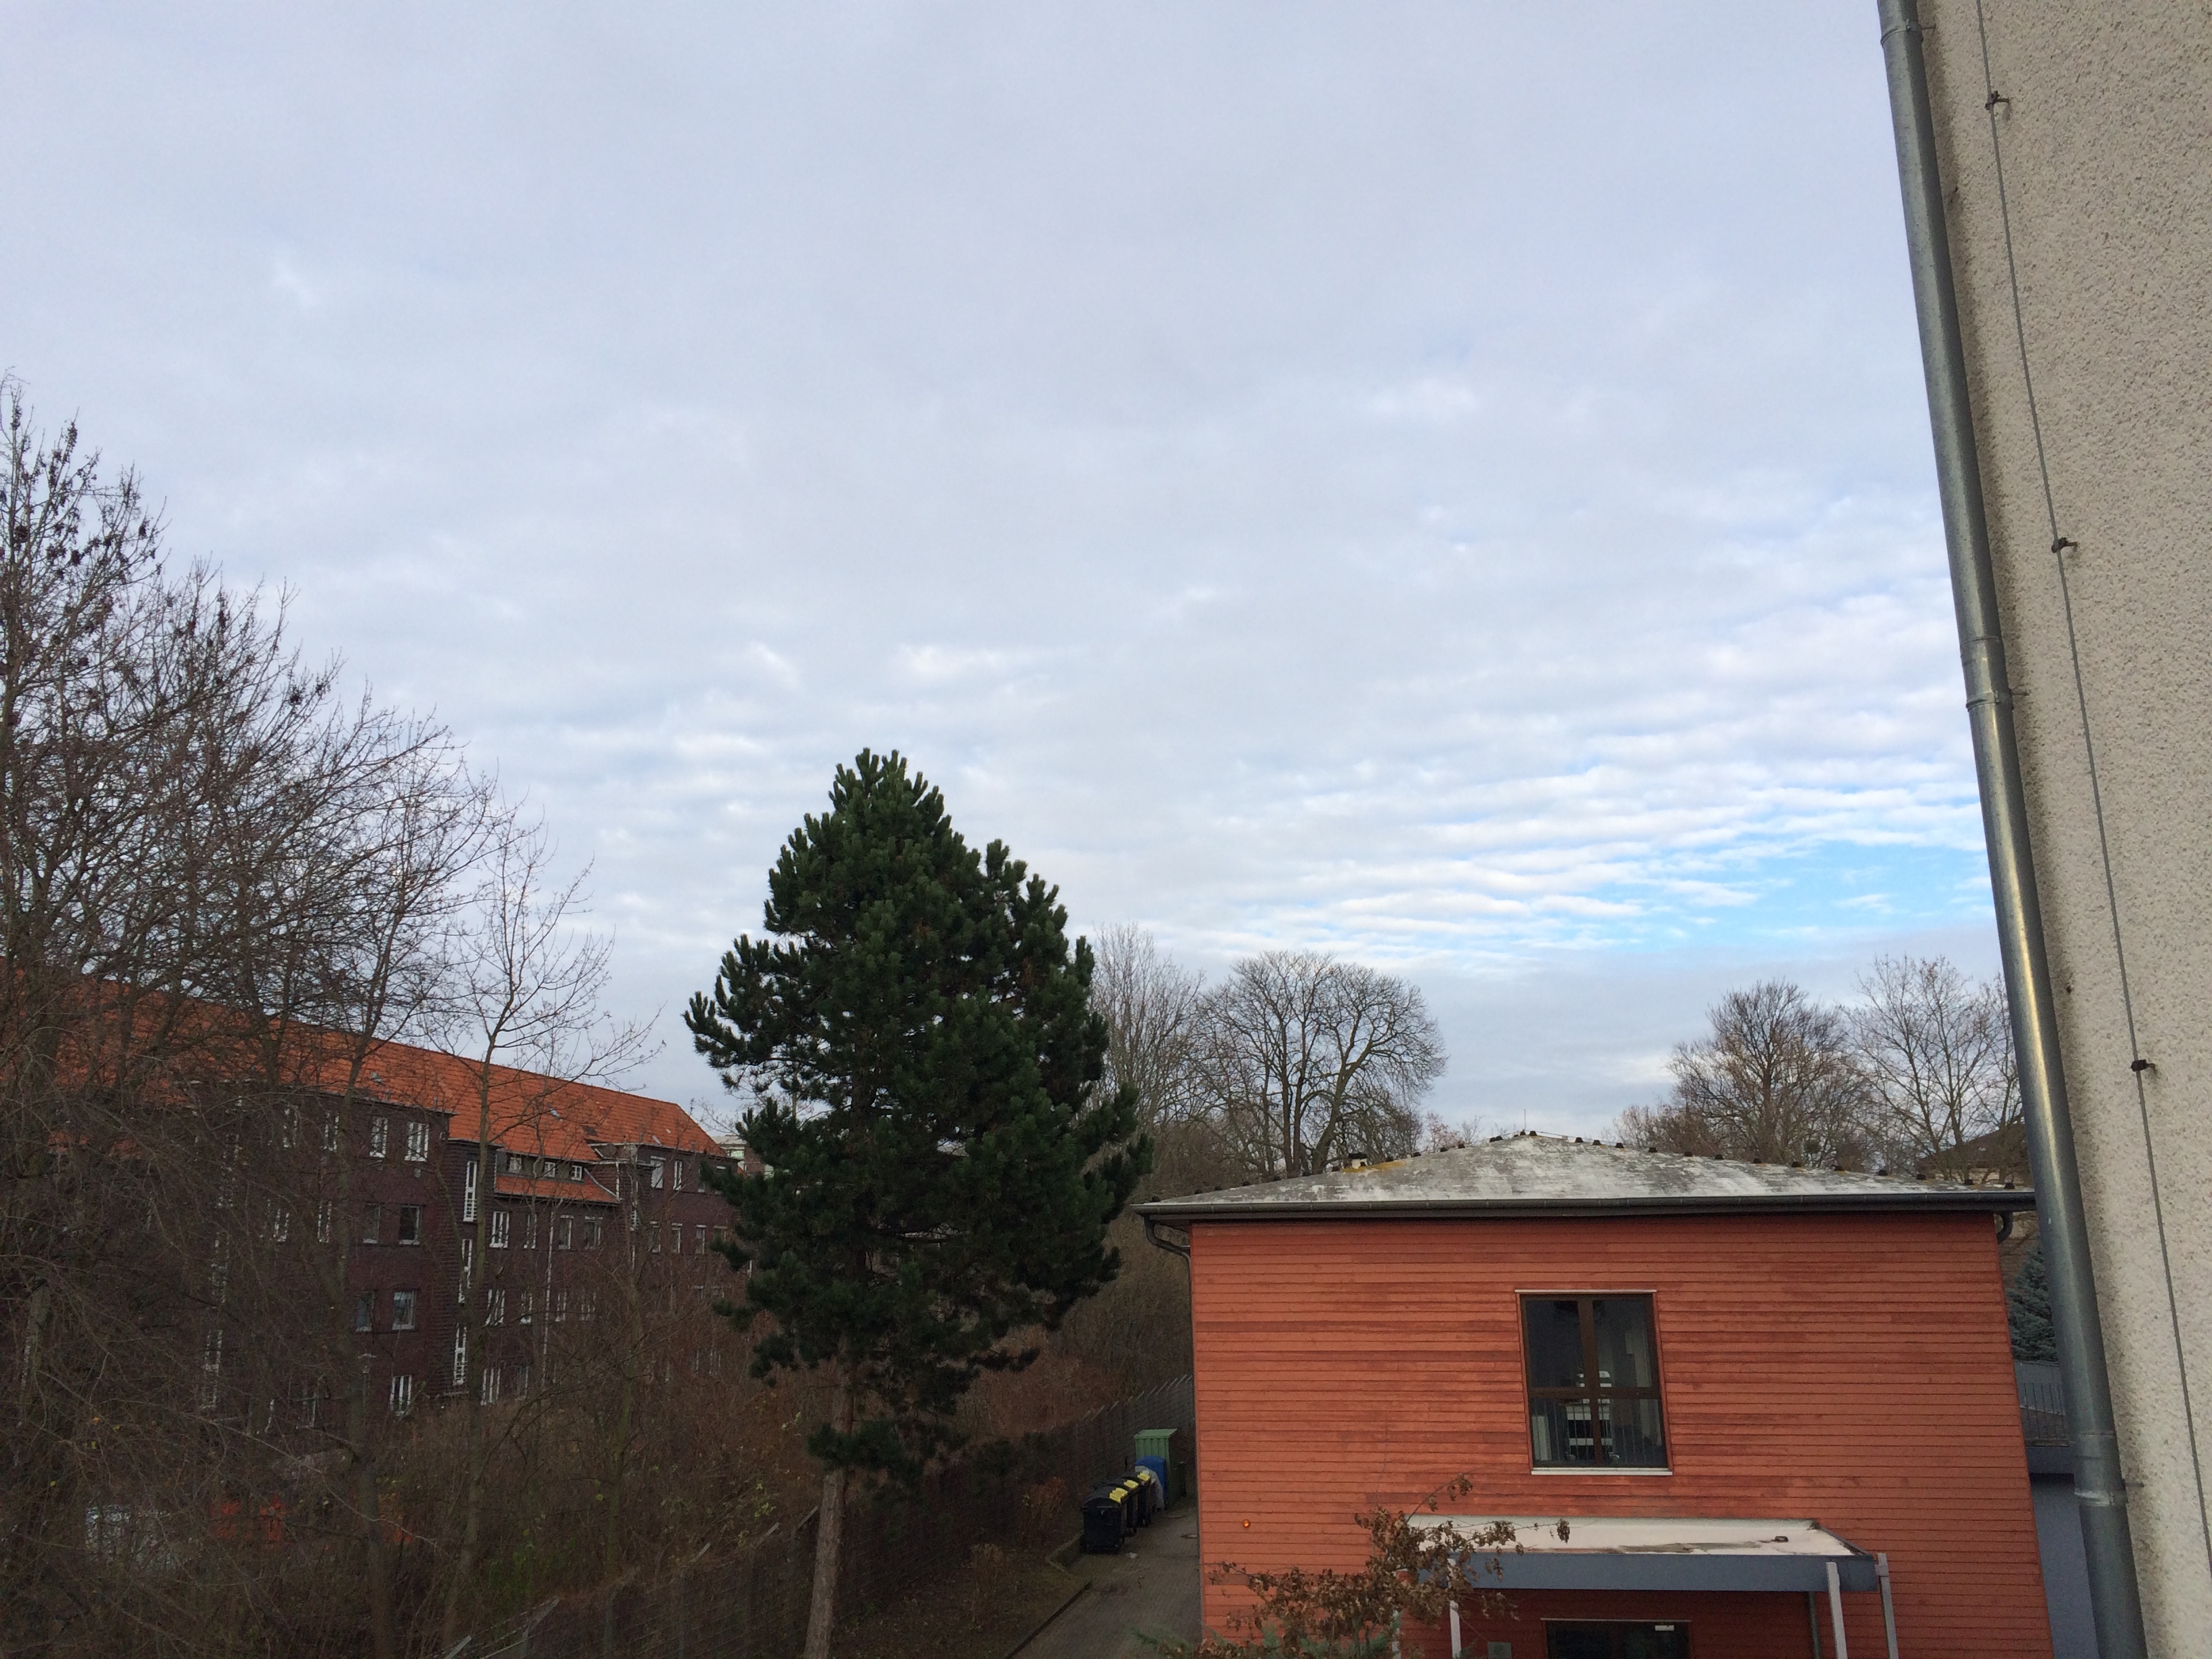
\includegraphics[width=0.49\textwidth]{wolkenNord}}
  \hfill
  \subfigure[Beschriftung 2\label{fig:wolkenSued}]
  {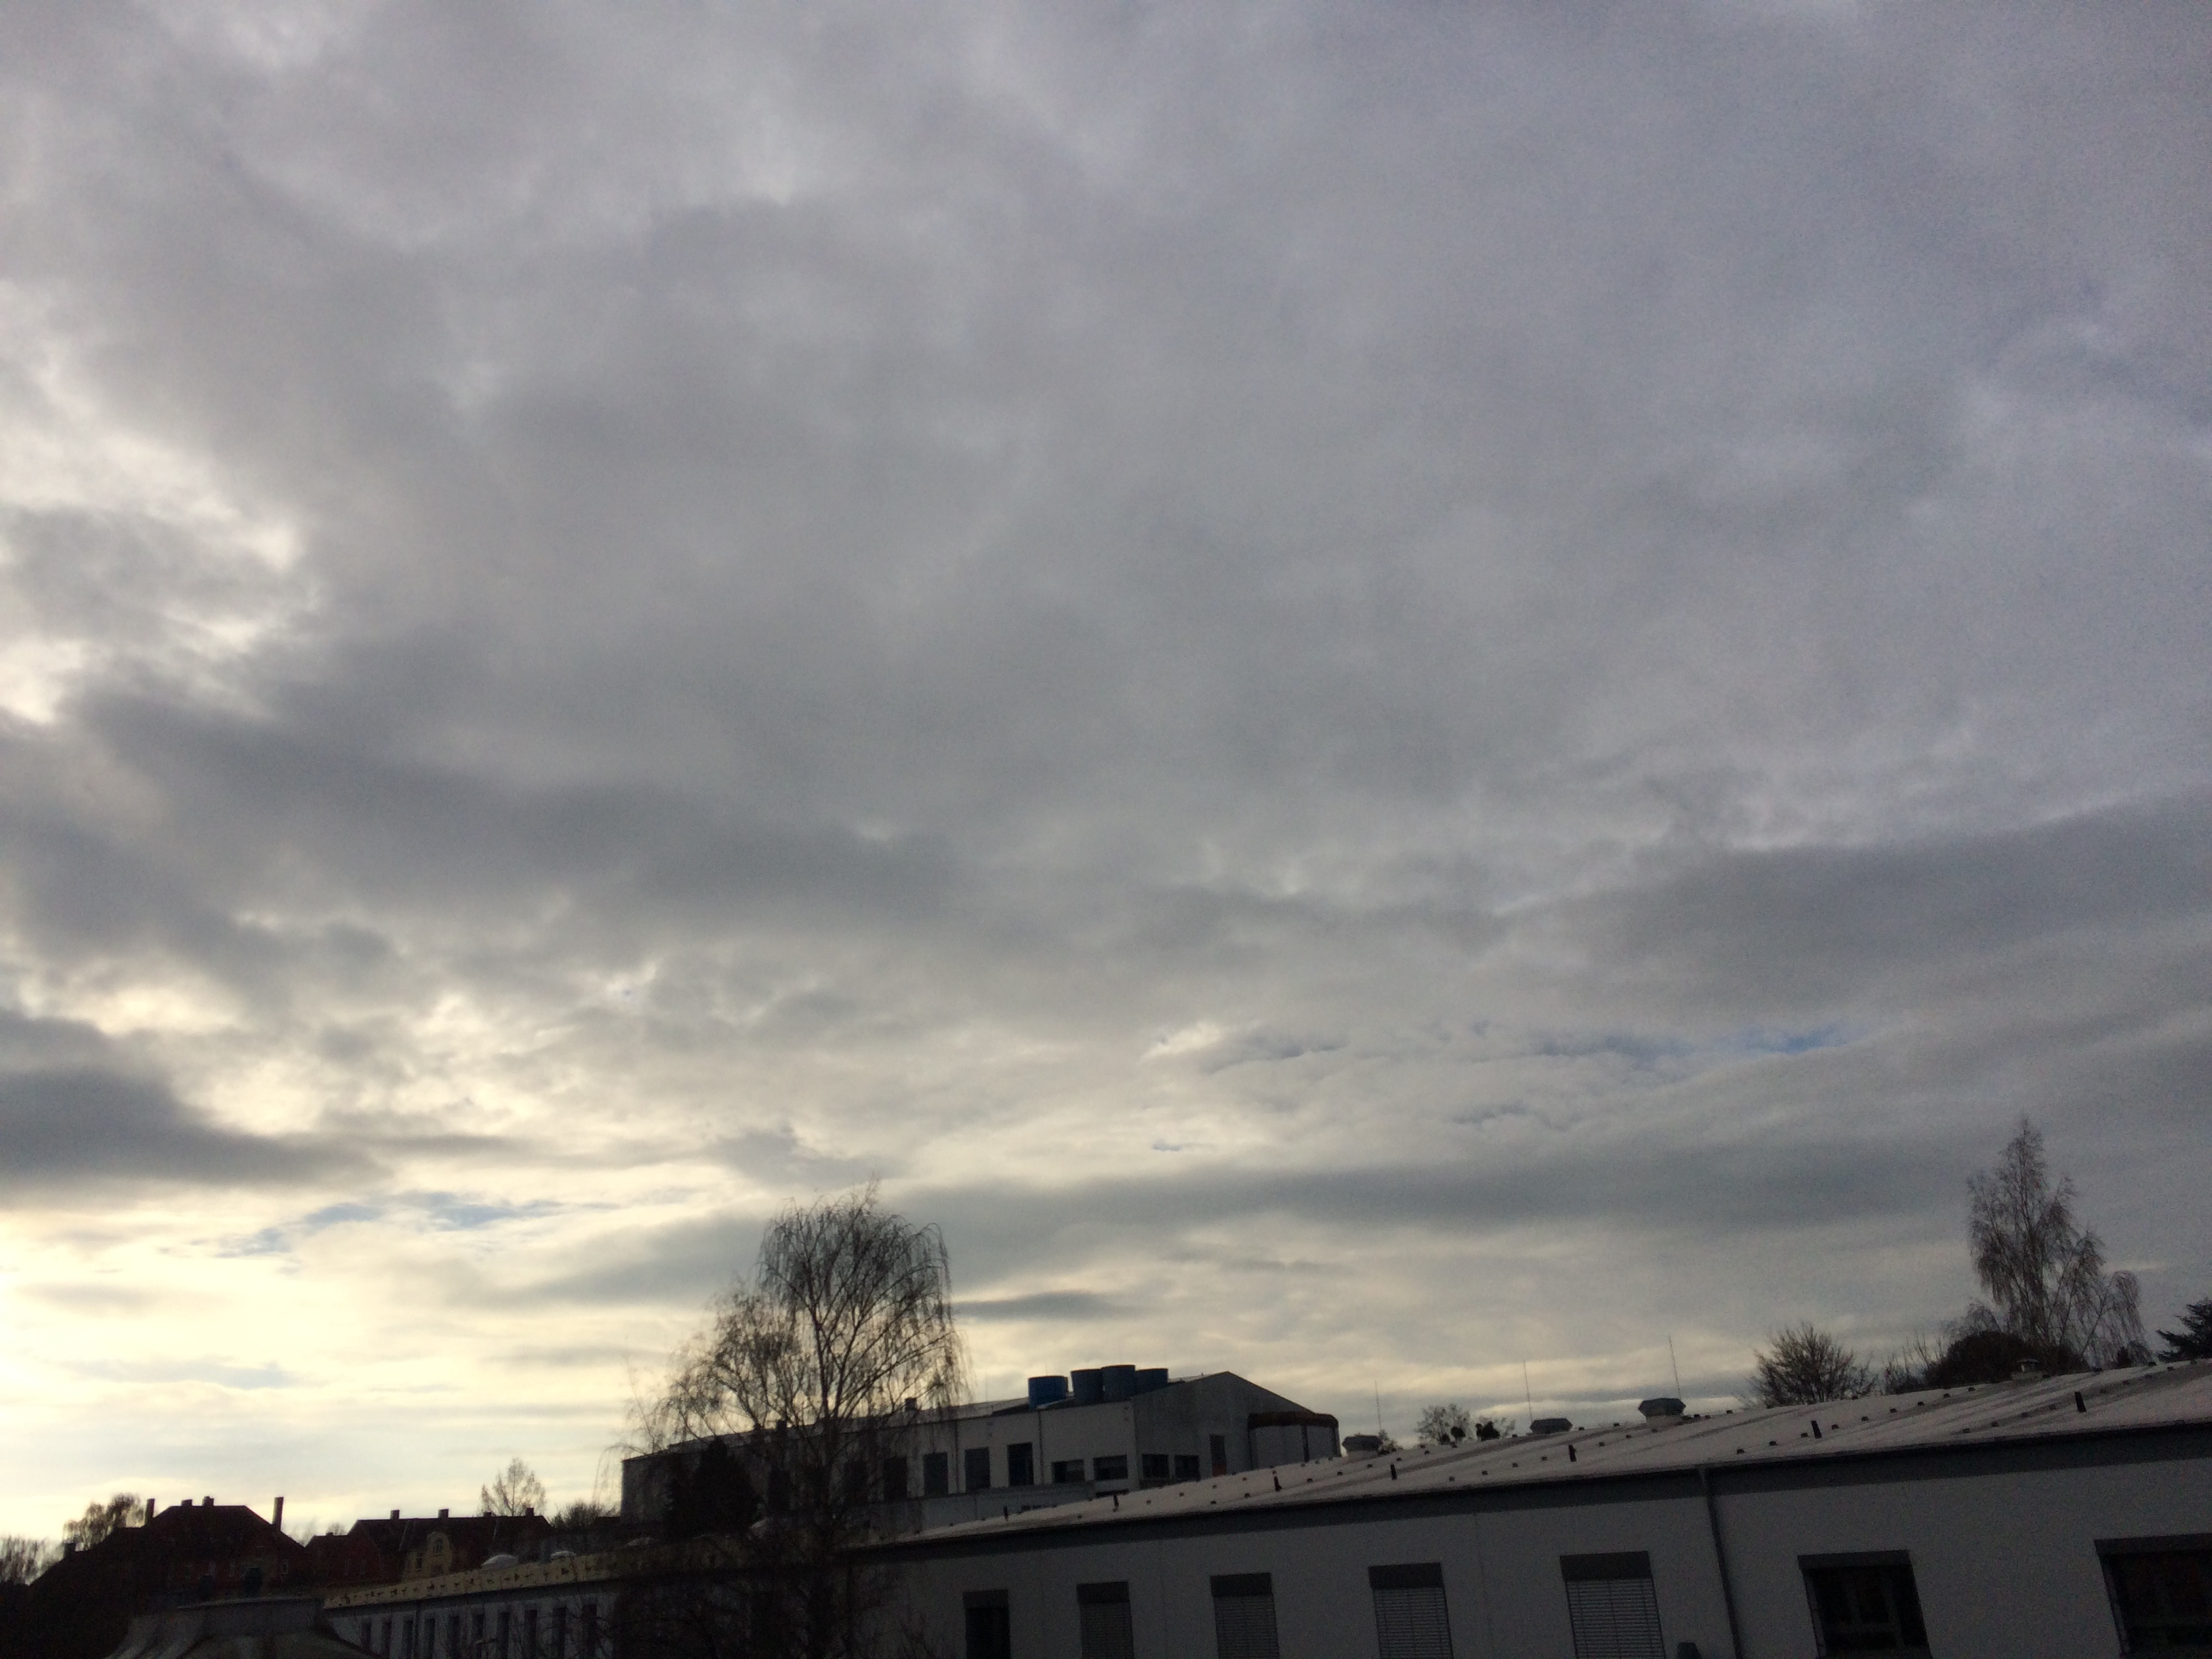
\includegraphics[width=0.49\textwidth]{wolkenSued}}
  \caption{Beschriftung allgemein}
  \label{fig:label-gesamt}
\end{figure}

\section{Aktuelle Wetterkarten}
Die Windstille war auch auf der Wetterkarte zu erkennen, da im Bereich von Göttingen die Dichte der Isobaren sehr gering war.
Diese deuteten auf eine vorherrschende Windrichtung von Westen her hin.
Die Warmfront, welche vor kurzem über Göttingen gezogen ist, bringt relativ warme Temperaturen.
Das Hochdruckgebiet über Südeuropa bringt durch die Zirkulation im Uhrzeigersinn warme, feuchte Luft zu uns.
Da es sehr stark ist ($\SI{1040}{\hecto\pascal}$), ist zu vermuten, dass die Kaltfront die Warmfront zunächst nicht einholen kann, da sie nicht über das Hochdruckgebiet kommt.
Deshalb wird die gesamte Front vermutlich Richtung Osten weggetrieben.

In der Vorschau der nächsten Wochen ist zu erkennen, dass bis ca. 15.12. das Wetter überwiegend durch Hochdruckgebiete über Südeuropa dominiert wird.
Am 13.12. wird jedoch vermutlich ein Ausläufer eines Tiefdruckgebietes über Skandinavien uns kalte feuchte Luft bringen.






\section{Diskussion}
\label{sec:diskussion}

\bibliography{literatur}
\bibliographystyle{babalpha}
\end{document}
